\documentclass{article}
\usepackage[a4paper]{geometry}
\usepackage{fancyhdr} 
\usepackage{tikz}
\pagestyle{fancy}
\lhead{Lagebeziehungen zwischen zwei Geraden}
\rhead{August 2025}
\begin{document}
 
\newcommand{\vect}[1]{\overrightarrow{#1}}
  
\section{Lagebeziehungen zwischen zwei Geraden}
Die Lagebeziehung zweier Geraden beschreibt, wie sie zueinander im Raum stehen. Dabei gibt es vier Möglichkeiten.
\begin{description}
 \item[Schneidung] Wenn zwei Geraden genau einen Schnittpunkt haben, schneiden sie sich. Dies impliziert, dass die Richtungsvektoren dessen Parametergleichungen nicht kollinear zueinander sind.
 \item[identisch] Teilen zwei Geraden sich alle ihre Punkte, sind sie identisch. Dies kann ermittelt werden, indem es entweder undendlich viele Lösungen beim LGS gibt oder es mindestens einen Schnittpunkt gibt und die Richtungsvektoren kollinear sind.
 \item[echt parallel] Zeigen zwei Geraden in die gleiche Richtung, sind also kollinear, berühren sich aber nicht, sind sie echt parallel.
 \item[windschief] Wenn zwei Geraden nicht kollinear sind, sicher aber auch nicht schneiden, sind sie windschief.
\end{description}
 
\begin{center}
 \begin{tabular}{c c c c}
  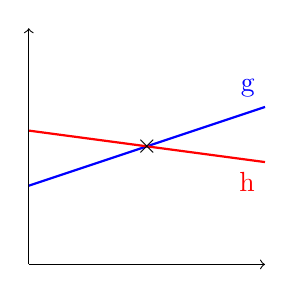
\begin{tikzpicture}
    \draw[thick, blue] (0, 1) -- ++(3, 1) node[above left] {g};
    \draw[thick, red] (0, 1.7) -- ++(3, -0.4) node[below left] {h};
   
    \draw (1.5, 1.5) node {$\times$};
  
    \draw[->] (0, 0) -- (3, 0); 
    \draw[->] (0, 0) -- (0, 3);
  \end{tikzpicture}  
  &
  \begin{tikzpicture}
    \draw[thick, blue, dashed] (0, 1.5) -- ++(3, 0) node[above left] {g};
    \draw[thick, red, dashed] (0.1, 1.5) -- ++(2.9, 0) node[below left] {h}; 
  
    \draw[->] (0, 0) -- (3, 0); 
    \draw[->] (0, 0) -- (0, 3);
  \end{tikzpicture}
  &
  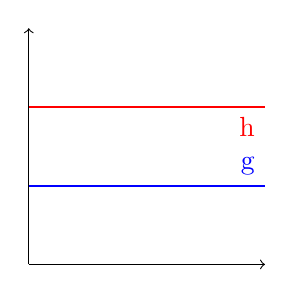
\begin{tikzpicture}
    \draw[thick, blue] (0, 1) -- ++(3, 0) node[above left] {g};
    \draw[thick, red] (0, 2) -- ++(3, 0) node[below left] {h};
 
    \draw[->] (0, 0) -- (3, 0); 
    \draw[->] (0, 0) -- (0, 3);
  \end{tikzpicture}
  &
  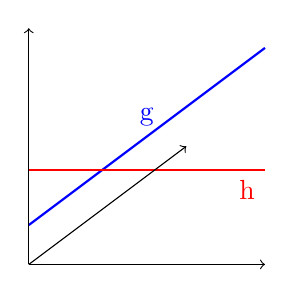
\begin{tikzpicture}
    \draw[thick,blue] (0,0.5) -- ++(3,0.75*3) node[midway, above] {g};
    \draw[thick,red] (0,1.2) -- ++(3,0) node[below left] {h};
 
    \draw[->] (0,0) -- (3,0);
    \draw[->] (0,0) -- (0,3);
    \draw[->] (0,0) -- (2,1.5);
  \end{tikzpicture}
  \\
  Schneidung & identisch & echt parallel & windschief
 \end{tabular} 
\end{center} 
 
 
\end{document} 
 
 
 
